% author Till Tantau
% modified by Truong Nhan Nguyen

\documentclass[tikz, border=10pt]{standalone}

\usepackage{tikz}
\usetikzlibrary{trees, snakes}
\usepackage{xcolor}

\tikzset{
    level 1/.style = {sibling angle=120},
    level 2/.style = {sibling angle=60},
    level 3/.style = {sibling angle=30},
    every node/.style = {fill},
    edge from parent/.style = {snake=expanding waves, segment length=1mm, segment angle=10, very thick, draw}
}

\begin{document}
    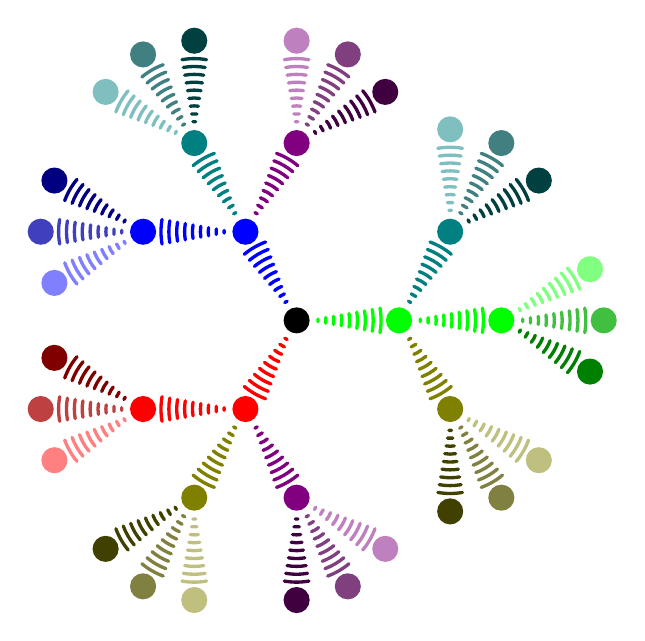
\begin{tikzpicture}[grow cyclic, shape=circle, level distance=13mm ,cap=round]
        \node {} child [color=\A] foreach \A in {red, green, blue} {
            node{} child [color=\A!50!\B] foreach \B in {red, green, blue}{
                node{} child[color=\A!50!\B!50!\C] foreach \C in {black, gray, white}{
                    node{}
                }
            }
        };
    \end{tikzpicture}
\end{document}